\documentclass[compress]{beamer}
\usepackage{ifthen,verbatim}

\newcommand{\isnote}{}
\xdefinecolor{lightyellow}{rgb}{1.,1.,0.25}
\xdefinecolor{darkblue}{rgb}{0.1,0.1,0.7}

%% Uncomment this to get annotations
%% \def\notes{\addtocounter{page}{-1}
%%            \renewcommand{\isnote}{*}
%% 	   \beamertemplateshadingbackground{lightyellow}{white}
%%            \begin{frame}
%%            \frametitle{Notes for the previous page (page \insertpagenumber)}
%%            \itemize}
%% \def\endnotes{\enditemize
%% 	      \end{frame}
%%               \beamertemplateshadingbackground{white}{white}
%%               \renewcommand{\isnote}{}}

%% Uncomment this to not get annotations
\def\notes{\comment}
\def\endnotes{\endcomment}

\setbeamertemplate{navigation symbols}{}
\setbeamertemplate{headline}{\mbox{ } \hfill
\begin{minipage}{5.5 cm}
\vspace{-0.75 cm} \small
\end{minipage} \hfill
\begin{minipage}{4.5 cm}
\vspace{-0.75 cm} \small
\begin{flushright}
\ifthenelse{\equal{\insertpagenumber}{1}}{}{Jim Pivarski \hspace{0.2 cm} \insertpagenumber\isnote/\pageref{numpages}}
\end{flushright}
\end{minipage}\mbox{\hspace{0.2 cm}}\includegraphics[height=1 cm]{../cmslogo} \hspace{0.1 cm} \includegraphics[height=1 cm]{../tamulogo} \hspace{0.01 cm} \vspace{-1.05 cm}}

\begin{document}
\begin{frame}
\vfill
\begin{center}
\textcolor{darkblue}{\Large Alignment of the CMS muon system with tracks}

\vfill
\begin{center}
\large
\textcolor{darkblue}{Jim Pivarski}

\scriptsize
\vspace{0.25 cm}
{\it Texas A\&M University}

\vspace{0.75 cm}
\small
\textcolor{darkblue}{on behalf of the CMS Collaboration}
\end{center}

\vfill
30 July, 2009

\end{center}
\end{frame}

%% \begin{notes}
%% \item This is the annotated version of my talk.
%% \item If you want the version that I am presenting, download the one
%% labeled ``slides'' on Indico (or just ignore these yellow pages).
%% \item The annotated version is provided for extra detail and a written
%% record of comments that I intend to make orally.
%% \item Yellow notes refer to the content on the {\it previous} page.
%% \item All other slides are identical for the two versions.
%% \end{notes}

\small

\begin{frame}
\frametitle{Outline}
\begin{itemize}\setlength{\itemsep}{0.35 cm}
\item Motivation for muon alignment

\item Quick overview of the CMS muon system

\item Alignment strategies

\item Endcap results with 2008 LHC beam-halo

\item Barrel results with CRAFT cosmic rays
\end{itemize}
%% \hspace{-0.83 cm} \textcolor{darkblue}{\Large Outline2}

\vfill
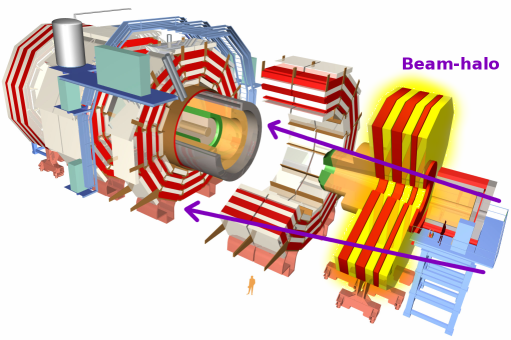
\includegraphics[width=0.47\linewidth]{CMS_exploded_endcap.png} \hfill 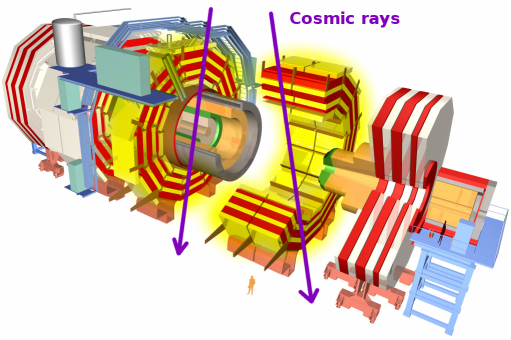
\includegraphics[width=0.47\linewidth]{CMS_exploded_barrel.png}
\end{frame}

\begin{frame}
\frametitle{Example physics case}

$Z' \to \mu\mu$ peak significance depends on resolution, and hence alignment

\vfill 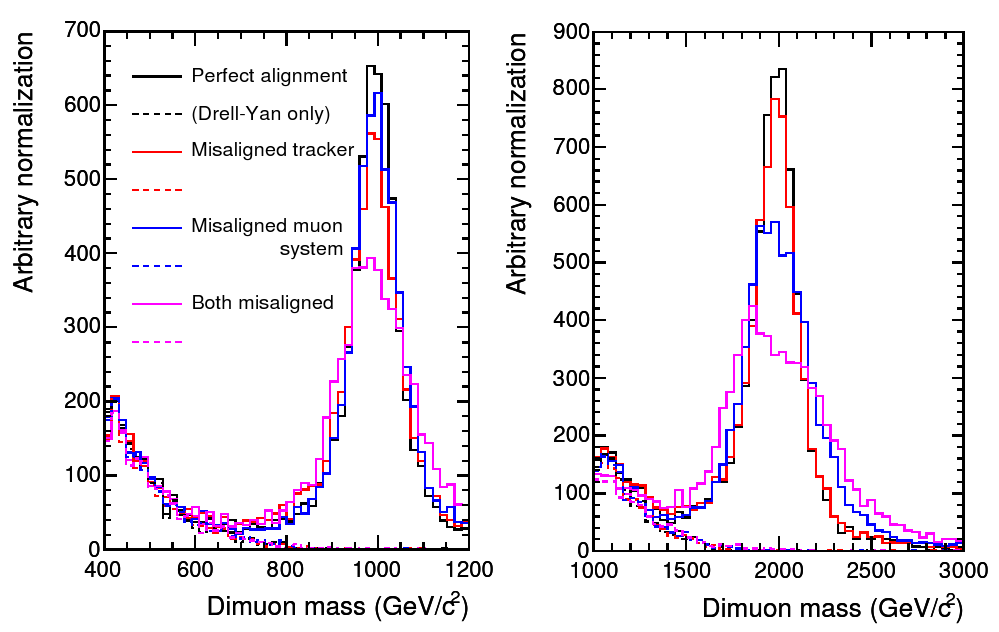
\includegraphics[width=\linewidth]{misaligned_spectra.png}

Importance of \textcolor{blue}{muon alignment (blue)} increases with muon energy
\end{frame}

\begin{frame}
\frametitle{CMS muon system}

\begin{itemize}
\item Tracking in modular chambers: 6 to 12 layers each
\item Global track formed from chambers' segments and \mbox{the silicon tracker\hspace{-1 cm}}
\end{itemize}

\begin{columns}
\column{0.7\linewidth}
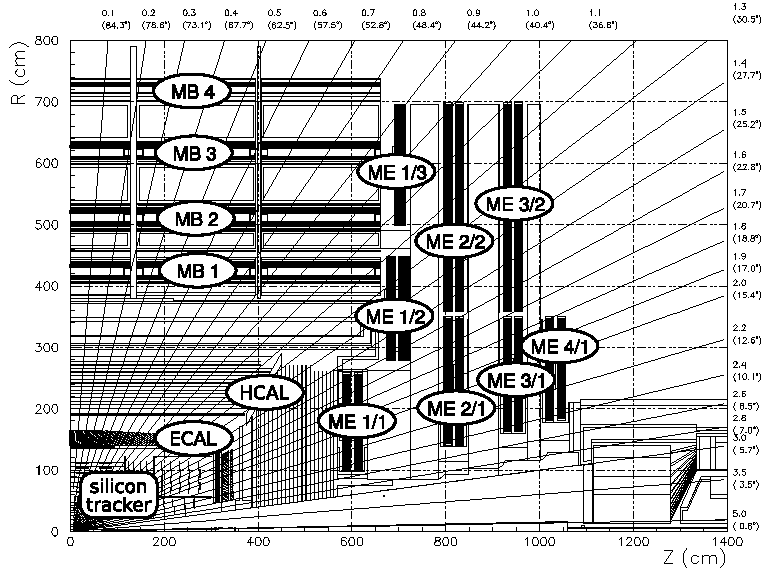
\includegraphics[width=\linewidth]{muon_system_labeled.pdf}

\column{0.3\linewidth}
\begin{itemize}
\item Barrel \mbox{(drift tube)} chambers grouped into 4~radial stations, 5~longitudinal wheels
\item Endcap \mbox{(cathode strip)} chambers grouped into 8~rings per endcap
\end{itemize}
\end{columns}

\begin{itemize}
\item This talk will be about aligning the individual chambers
\item Target for alignment is scale of $r\phi$ hit resolutions: $\mathcal{O}(\mbox{100--300~$\mu$m})$
\end{itemize}
\end{frame}

\begin{frame}
\frametitle{Alignment Strategy}

\begin{itemize}\setlength{\itemsep}{0.35 cm}
\item \textcolor{darkblue}{Consideration:} Tracks measured with high precision in the silicon tracker, then
  pass through thick layers of iron (solenoid return yoke)
\begin{itemize}\setlength{\itemsep}{0.2 cm}
\item resolution of global tracks is dominated by tracker data \\ (for $p_T \lesssim 200$~GeV in barrel, $p_T \lesssim 500$~GeV in endcap)
\item scattering in iron can be confused for misalignment \mbox{with a single\hspace{-2 cm}} \\ track, but scattering is random; misalignment is systematic
\end{itemize}

\vspace{0.5 cm}
\hfill 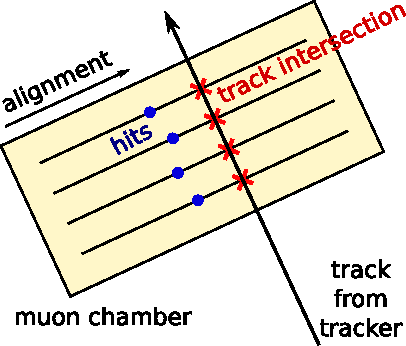
\includegraphics[height=3.3 cm]{hip_explanation.pdf}
\vspace{-3.5 cm}

\item \textcolor{darkblue}{Strategy:} fit tracks to the tracker only, \\ then propagate to the muon system
\begin{itemize}\setlength{\itemsep}{0.2 cm}
\item misalignment given by the {\it peak} \\ of the residuals distribution \\ (residual = track $-$ hit)
\item control for propagation effects: \\ material budget, $\vec{B}(\vec{x})$, etc. \\ have different dependencies on momentum and charge
\end{itemize}
\end{itemize}
\end{frame}

\begin{frame}
\frametitle{Alignment Strategy}

\begin{itemize}
\item \textcolor{darkblue}{Consideration:} no obstacles to track-fits inside the chambers
\begin{itemize}
\item gas volume with negligible scattering
\item low magnetic field: field lines follow iron yoke \mbox{between chambers\hspace{-1 cm}}
\end{itemize}

\hfill 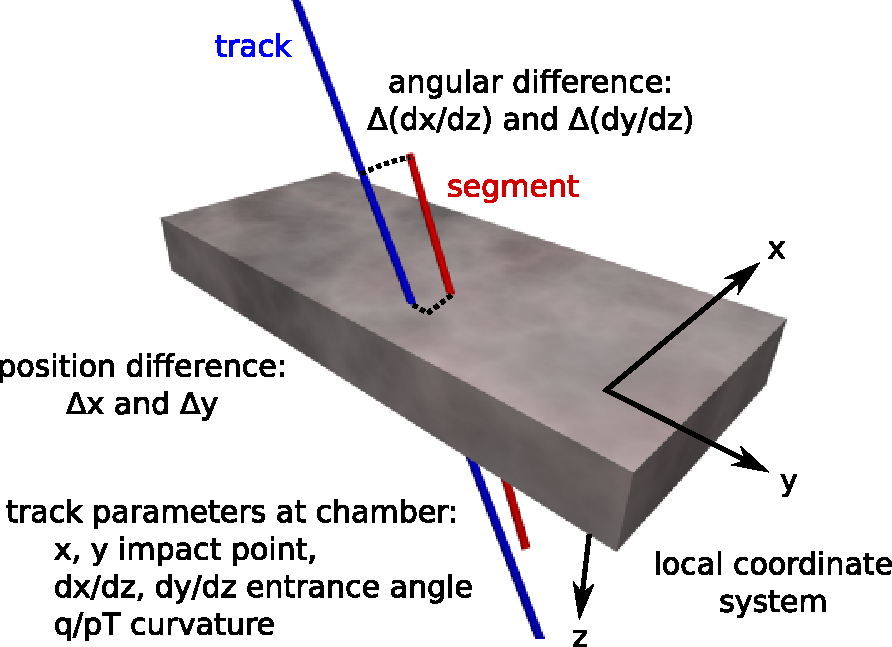
\includegraphics[width=0.6\linewidth]{dt_coordinates.pdf}
\vspace{-4.25 cm}

\item \textcolor{darkblue}{Strategy:} combine residuals into a \\ 2-D
  position difference and a \\ 2-D angle difference \\ (4-component ``residuals'')

\vspace{2.8 cm}
\begin{itemize}
\item more highly constrained than traditional approach
\item compute 6 rigid-body degrees of freedom (3~translations and
3~rotations) from inversion of $6\times 4$ matrix, rather than $6\times 2$
\end{itemize}
\end{itemize}
\end{frame}

\begin{frame}
\frametitle{Sample fits: \only<1>{Monte Carlo}\only<2>{real cosmic rays}}

\vspace{0.25 cm}
\begin{columns}
\column{0.5\linewidth}

\mbox{ } \hfill \textcolor{darkblue}{Before alignment} \hfill \mbox{ }

\only<1>{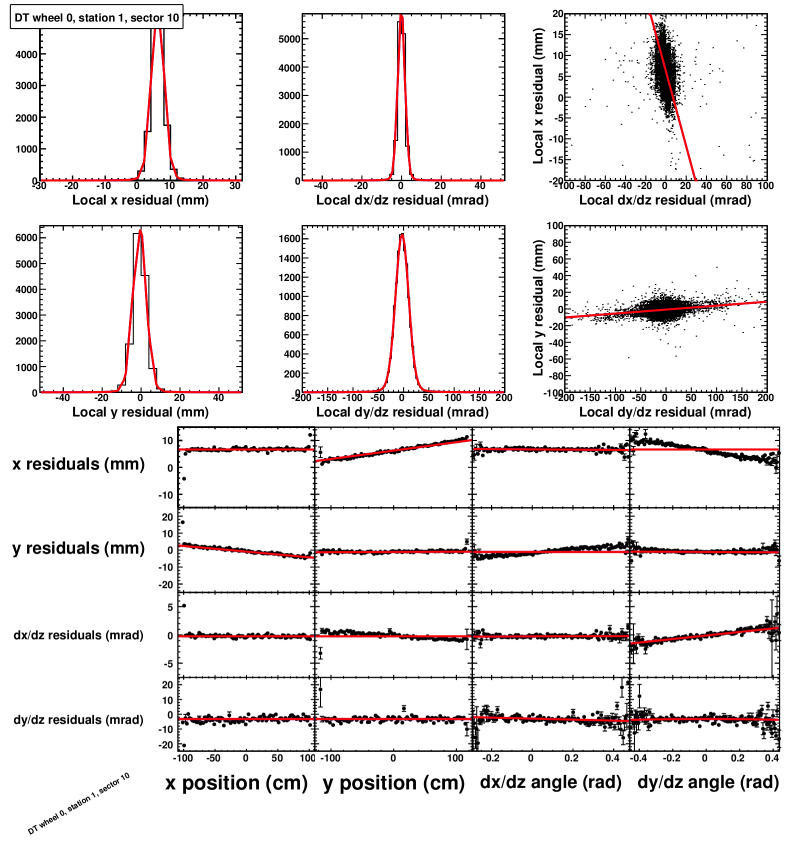
\includegraphics[width=\linewidth]{exampleMC_wh0st1sec10_before.png}}\only<2>{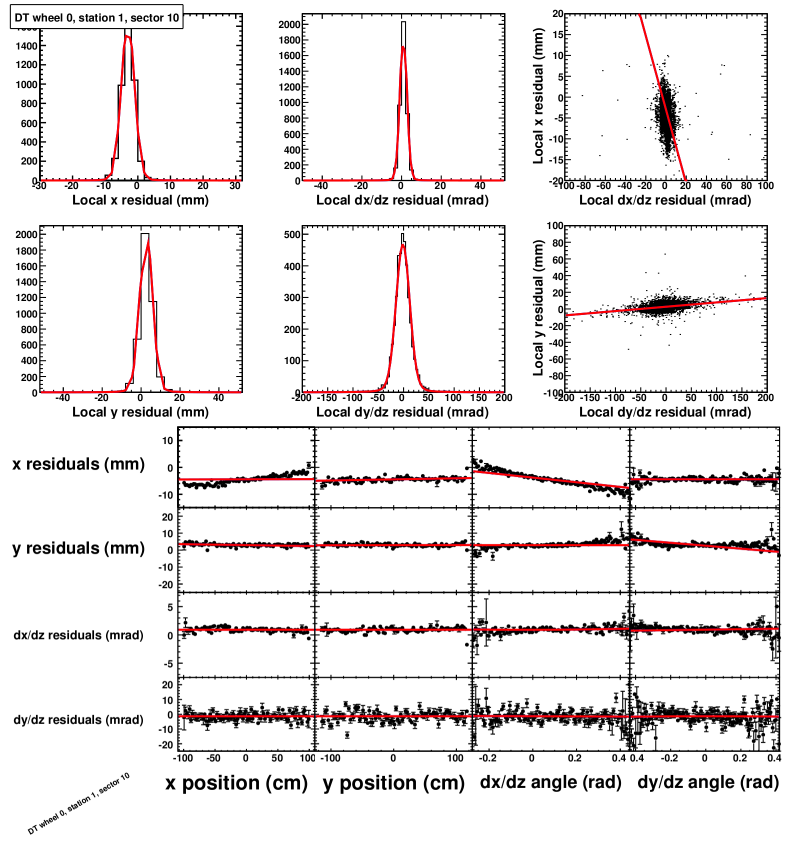
\includegraphics[width=\linewidth]{exampleData_wh0st1sec10_before.png}}

\column{0.5\linewidth}

\mbox{ } \hfill \textcolor{darkblue}{After alignment} \hfill \mbox{ }

\only<1>{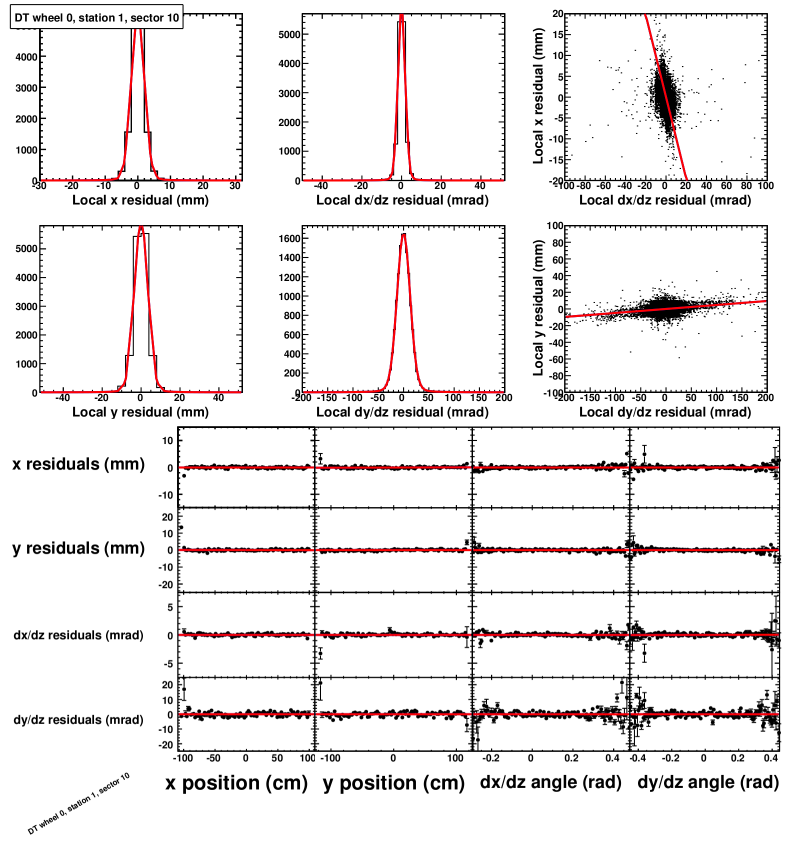
\includegraphics[width=\linewidth]{exampleMC_wh0st1sec10_after.png}}\only<2>{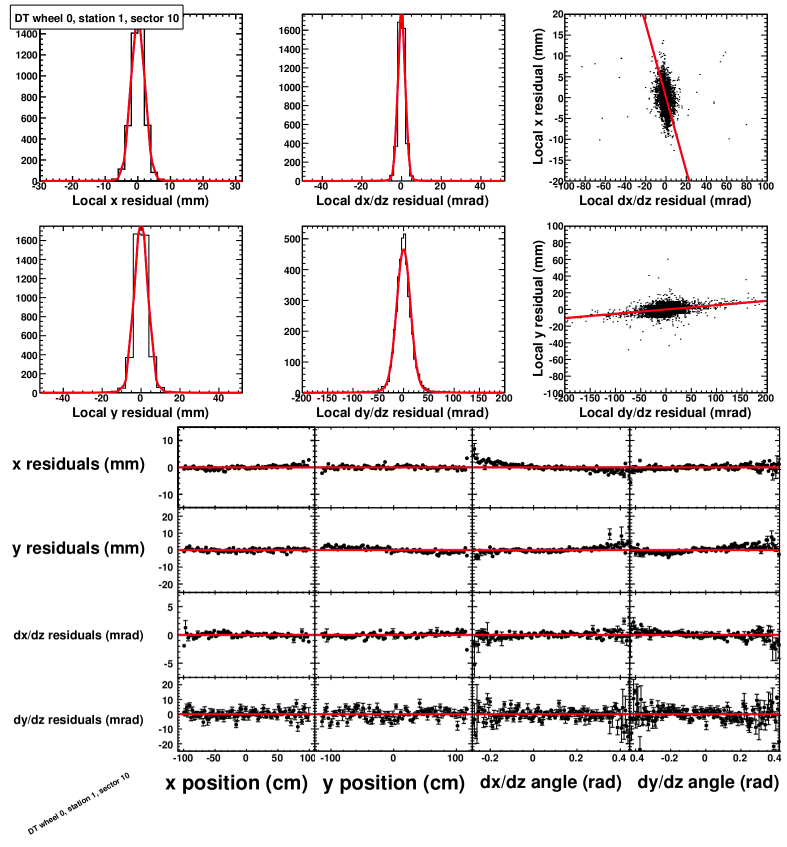
\includegraphics[width=\linewidth]{exampleData_wh0st1sec10_after.png}}

\end{columns}

\begin{itemize}
\item Projection of \textcolor{red}{fits (all parameters = 0 other than the one shown)} overlaid on {\it \only<1>{simulated}\only<2>{real}} data for \only<1>{one}\only<2>{the same} chamber
\item \only<1>{Method works well in Monte Carlo}\only<2>{Largely the same behavior in data; studying small discrepancies}
\end{itemize}
\end{frame}

\begin{frame}
\frametitle{Monte Carlo accuracy}

\begin{itemize}
\item Plot aligned-minus-true value of each of the 6 parameters for every chamber (histogram entries are chambers)
\begin{itemize}
\item achieved 100--300~$\mu$m goal in $r\phi$ (local $x$ coordinate: top-left)
\item systematics-dominated event sample
\end{itemize}
\end{itemize}

\vfill
\mbox{ } \hfill 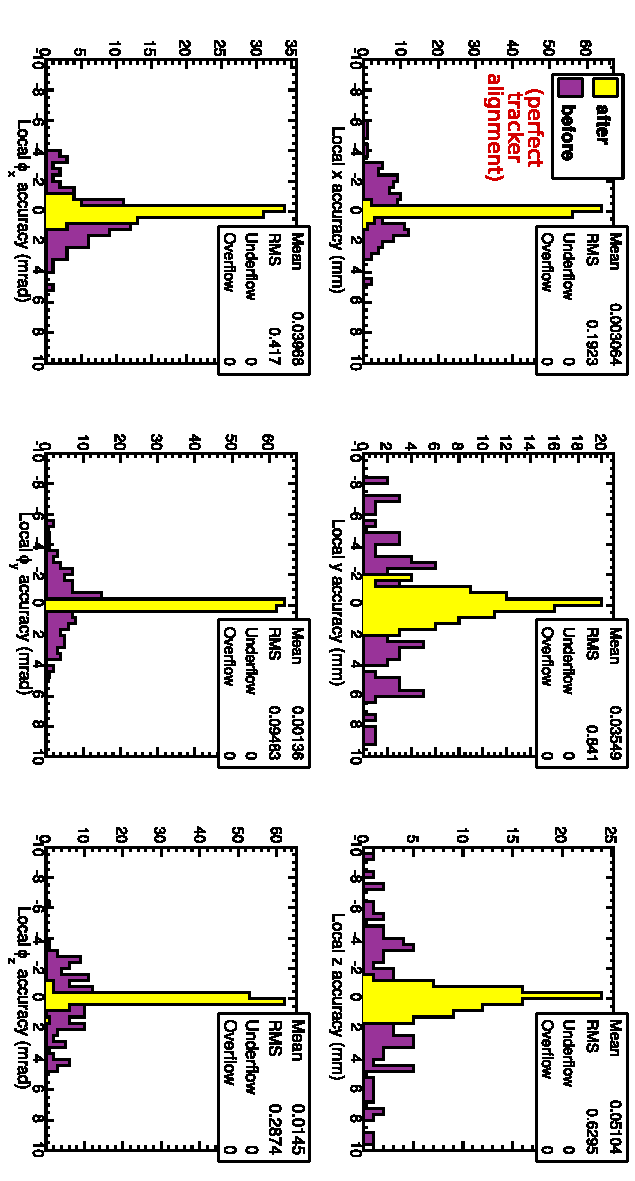
\includegraphics[height=0.9\linewidth, angle=90]{hip_MC_simple2.pdf} \hfill \mbox{ }

\vfill \scriptsize Note: this is a study of the muon alignment only,
given a perfectly-aligned silicon tracker for input tracks.
\end{frame}

\begin{frame}
\frametitle{Alignment Strategy}

\begin{itemize}\setlength{\itemsep}{0.25 cm}
\item \textcolor{darkblue}{Consideration:} Complimentary information available from global and local track propagations
\begin{itemize}\setlength{\itemsep}{0.2 cm}
\item propagation from the silicon tracker conveys information about the global CMS coordinate system
\item propagation from one chamber to its neighbor is less susceptible to scattering
\item partially-independent datasets from the same muons!
\end{itemize}

\item \textcolor{darkblue}{Strategy:} Develop alignment methods for both and cross-check

\hfill 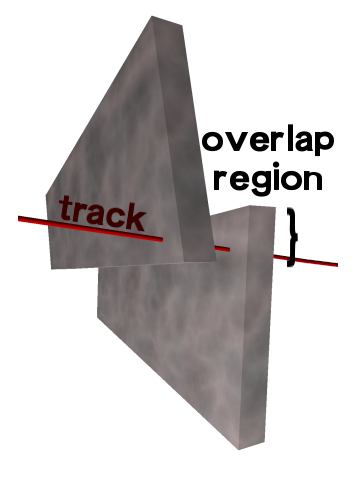
\includegraphics[height=3 cm]{overlaps.png}
\vspace{-3.3 cm}

\begin{itemize}\setlength{\itemsep}{0.2 cm}
\item in the endcap, Cathode Strip Chambers \\ (CSCs) overlap along their edges
\item propagate relative alignment information \\ through all overlapping CSC pairs
\item provides a complete alignment within \\ a consistent local coordinate system
\end{itemize}
\end{itemize}
\end{frame}

\begin{frame}
\frametitle{Alignment from CSC Overlaps}

\begin{columns}
\column{0.2\linewidth}
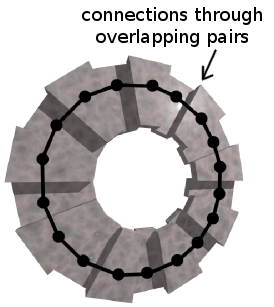
\includegraphics[width=1.25\linewidth]{matrix_description_onestation.png}

\column{0.4\linewidth}
\begin{itemize}
\item Align a ring of CSCs with only local tracks by solving a system of 18 or 36 equations (for 18, 36 chambers per ring)
\item Apply to 3 degrees of freedom
\end{itemize}

\column{0.35\linewidth}
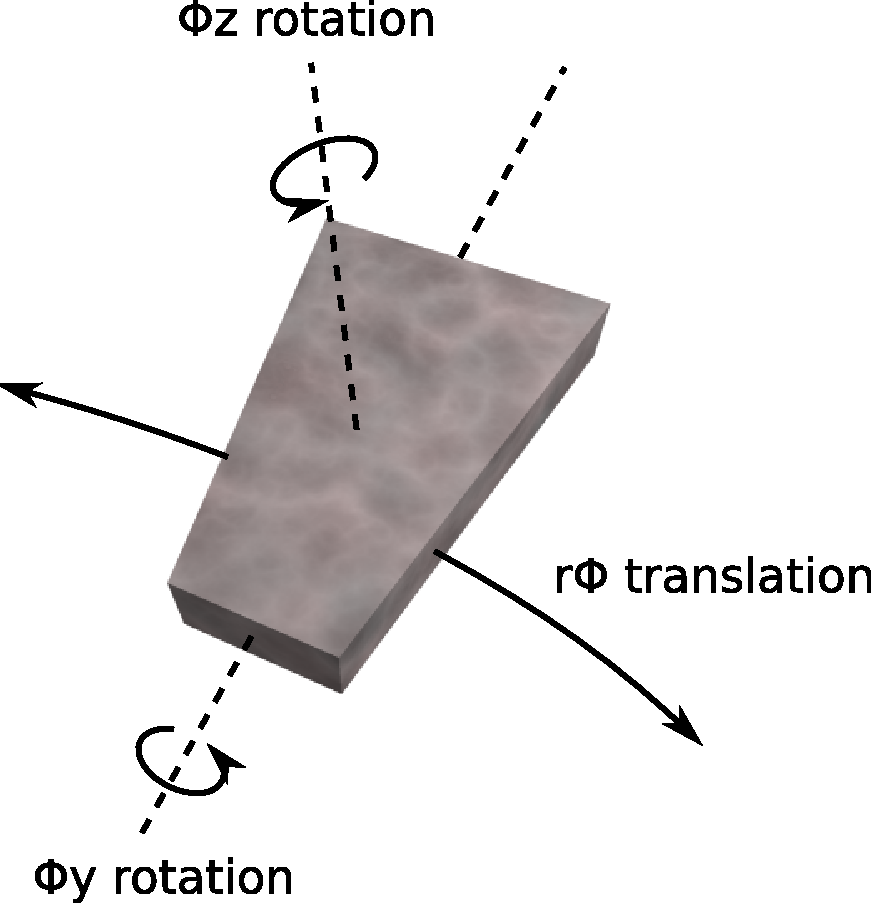
\includegraphics[width=\linewidth]{csc_coordinates.pdf}
\end{columns}

\hspace{-0.83 cm} \textcolor{darkblue}{\Large Monte Carlo accuracy} \hfill {\scriptsize (statistics limited, similar sample size as data)}

\vspace{0.25 cm}
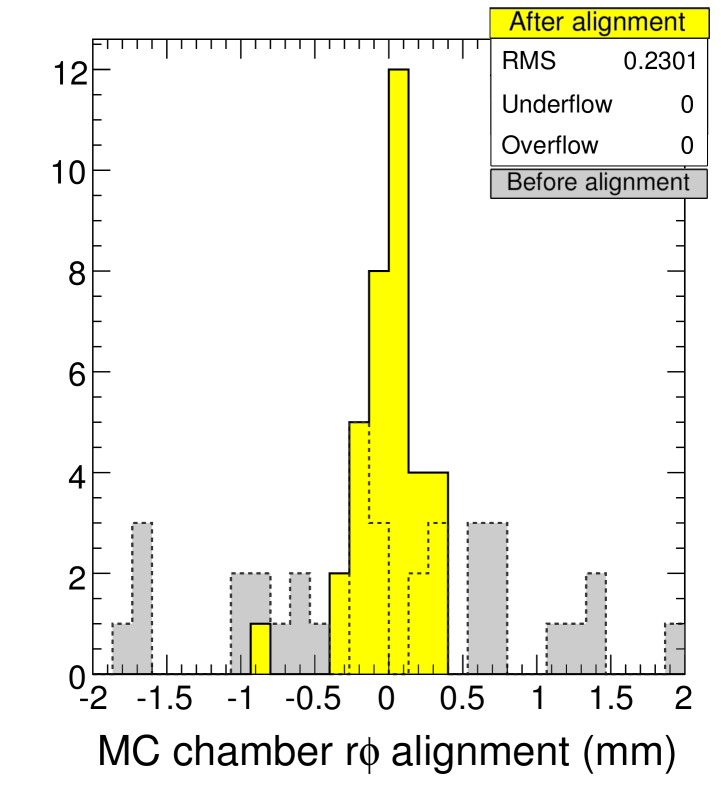
\includegraphics[width=0.33\linewidth]{mc_rphi.png}
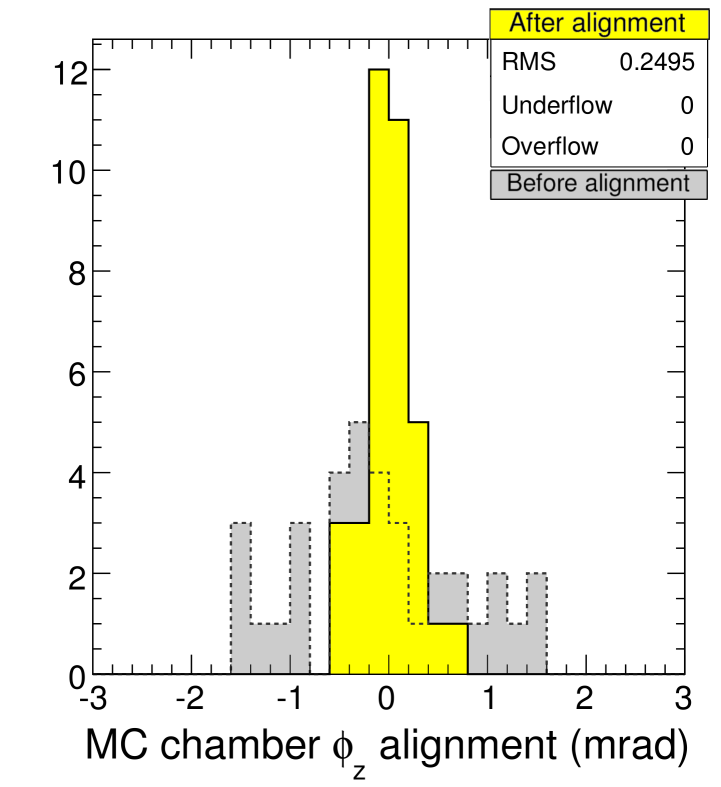
\includegraphics[width=0.33\linewidth]{mc_phiz.png}
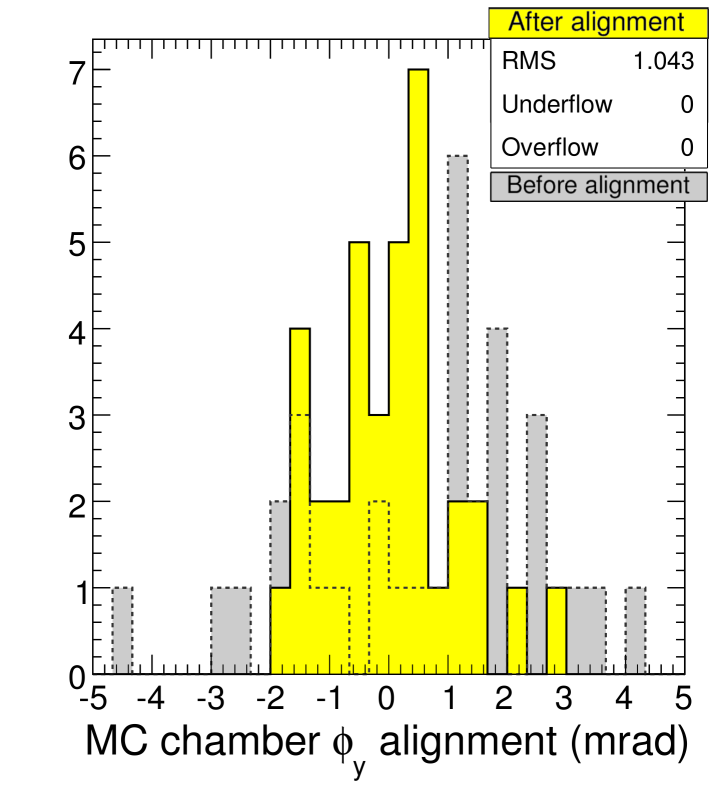
\includegraphics[width=0.33\linewidth]{mc_phiy.png}
\end{frame}

\begin{frame}
\frametitle{2008 LHC beam-halo data}

\begin{itemize}
\item Captured a total of 12 minutes of LHC muons, Sept 10--19, 2008
\item Enough to align CSC rings closest to the beamline \\ (33,000 events in overlapping edges)
\item Local alignment cross-checked by photogrammetry: measurements from a literal photograph of the detector
\end{itemize}

\vspace{0.2 cm}
\begin{columns}
\column{0.35\linewidth}
Both methods observed (expected) differences with respect to the design geometry, with high correlation

\column{0.65\linewidth}
\hspace{-1 cm} 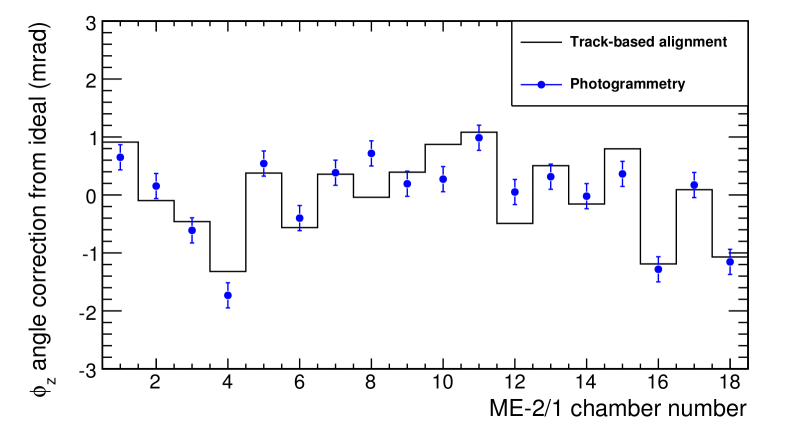
\includegraphics[width=1.1\linewidth]{data_correlations.png}
\end{columns}
\end{frame}

\begin{frame}
\frametitle{2008 LHC beam-halo data}

\vspace{0.2 cm}
\mbox{\hspace{-0.5 cm}\begin{minipage}{\linewidth}
\begin{itemize}
\item Chamber-by-chamber comparisons with photogrammetry (PG):
\begin{itemize}\setlength{\itemsep}{0.1 cm}
\item agreement with \textcolor{darkblue}{270~$\mu$m} position and \textcolor{darkblue}{0.35~mrad} \mbox{angular accuracy\hspace{-1 cm}}
\item for these chambers, intrinsic hit uncertainty is 166~$\mu$m
\item statistics-limited: reach $\sigma_{\mbox{\scriptsize align}} \lesssim \sigma_{\mbox{\scriptsize hits}}$ with an hour of beam
\end{itemize}
\end{itemize}
\end{minipage}}

\vspace{0.4 cm}
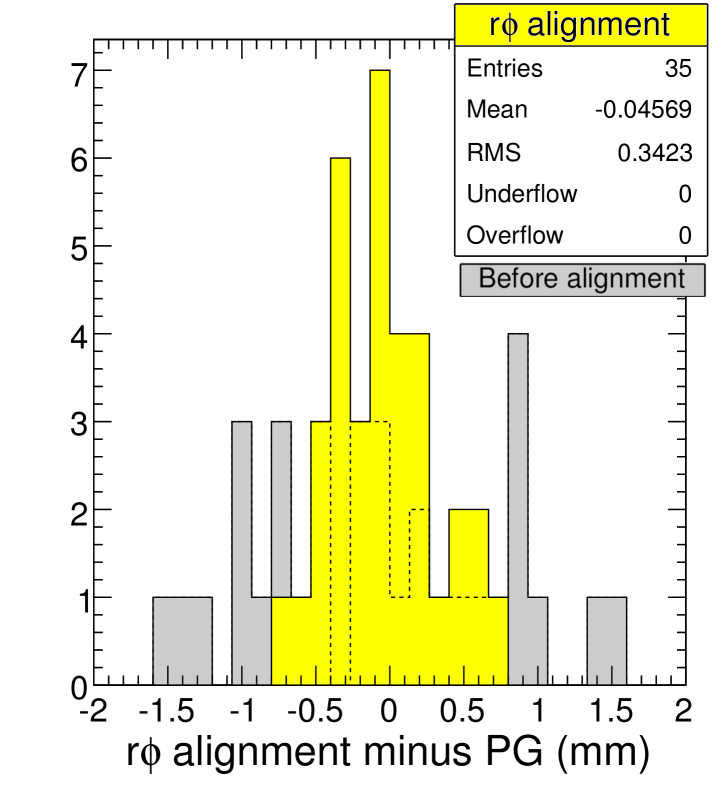
\includegraphics[width=0.5\linewidth]{data_rphi.png}
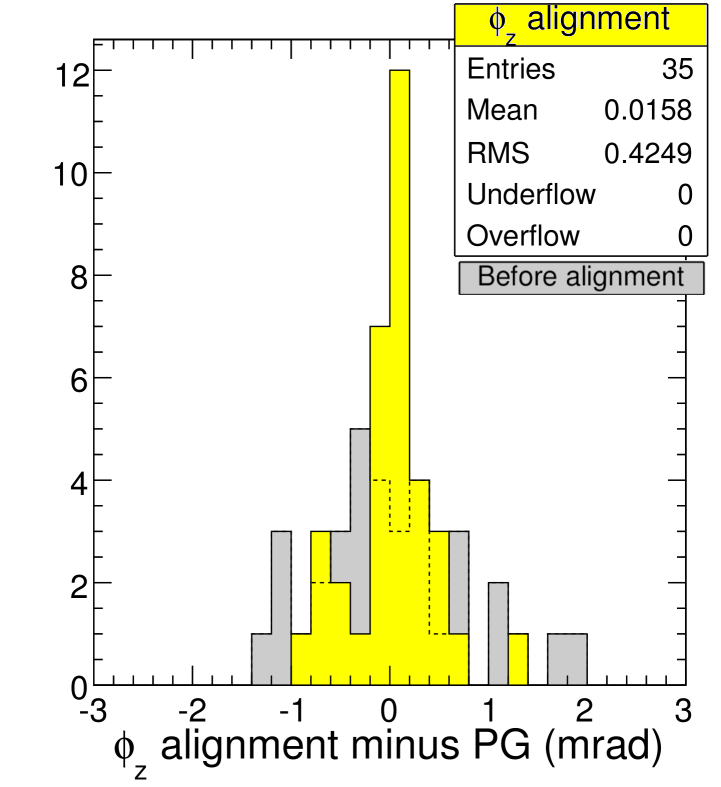
\includegraphics[width=0.5\linewidth]{data_phiz.png}
\end{frame}

\begin{frame}
\frametitle{CRAFT cosmic ray data}

\begin{itemize}\setlength{\itemsep}{1 cm}
\item Cosmic Rays At Four Tesla (CRAFT): 1 month of cosmic rays
\begin{itemize}
\item all systems taking data concurrently: can align major subsystems relative to one another
\item solenoid at full field (3.8~T): can select high-momentum tracks
\end{itemize}

\vspace{0.25 cm}

\hfill 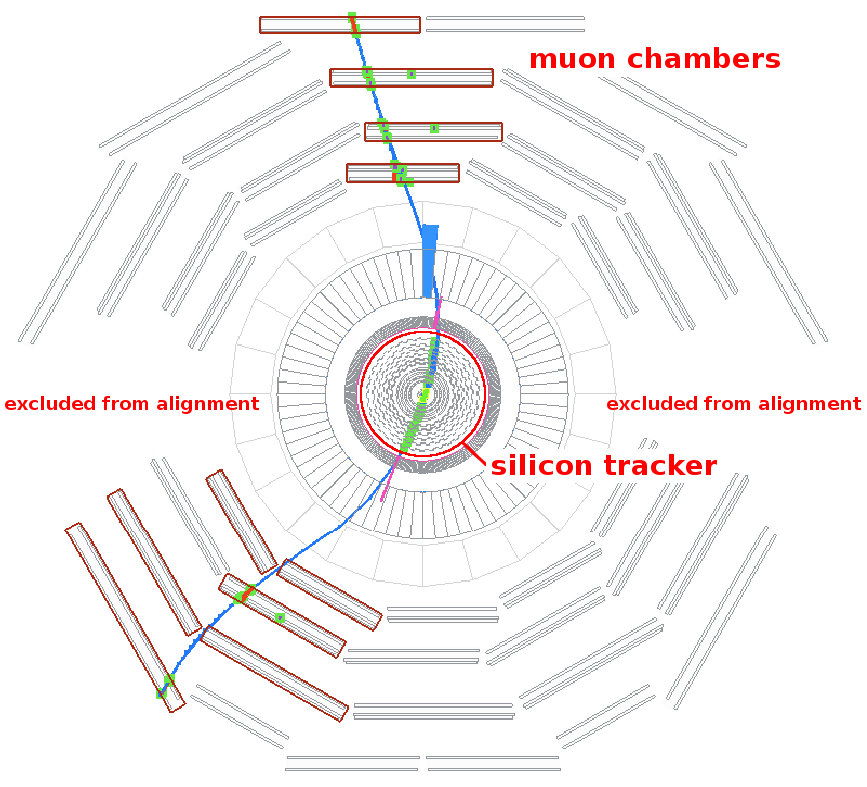
\includegraphics[width=0.5\linewidth]{event_display.png}
\vspace{-5 cm}

\item Applied global alignment procedure \\ to top and bottom of barrel \\ (central 3 wheels, 10/12 sectors, \\ due to vertical distribution \\ of cosmic rays)

\item Data and MC are both \\ systematics-limited in most chambers
\end{itemize}
\end{frame}

\begin{frame}
\frametitle{CRAFT cosmic ray data}

\begin{itemize}
\item Cross-check of global alignment with local data
\begin{itemize}\setlength{\itemsep}{0.2 cm}
\item propagate chamber segments through only one layer of iron with
  aligned geometry, check for consistency
\item RMS of differences: 0.42~mm, 0.18~mrad for \mbox{innermost chambers\hspace{-1 cm}}
\end{itemize}

\end{itemize}

\vfill
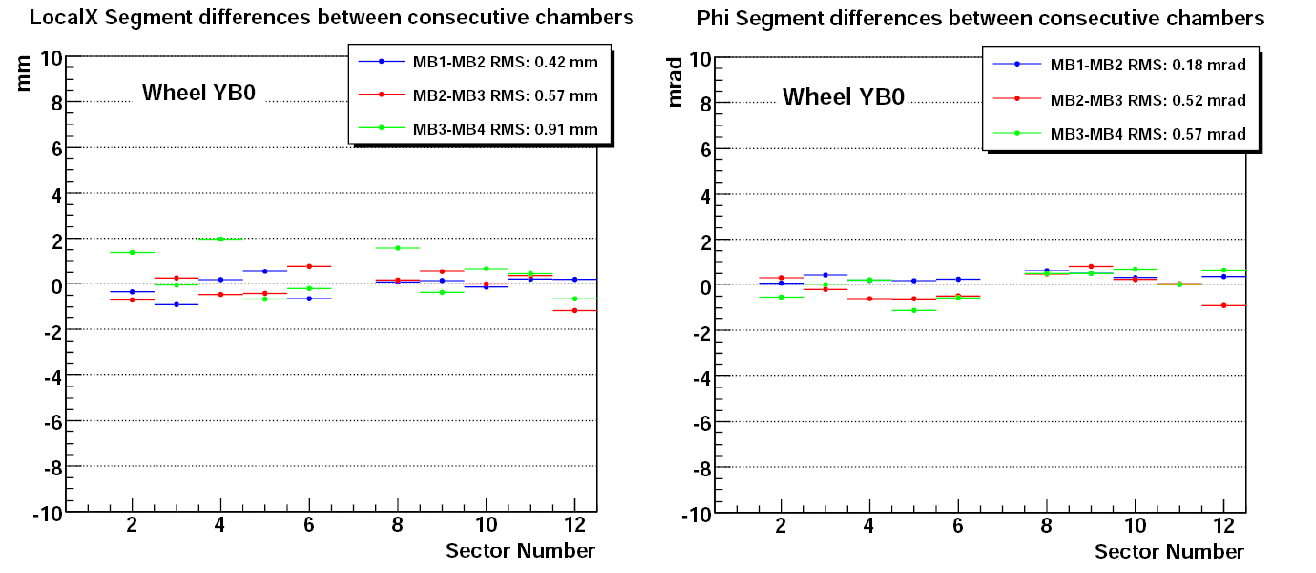
\includegraphics[width=\linewidth]{segment_extrapolation.png}
\end{frame}

\begin{frame}
\frametitle{CRAFT cosmic ray data}

\begin{itemize}
\item High-level test: split each cosmic ray into two LHC-like halves, fit top and bottom independently
\begin{itemize}
\item any mismatch in $1/p_T$ is purely instrumental
\item select $p_T \gtrsim 200$~GeV to emphasize contribution of the muon alignment (long lever arm for resolution of small sagitta)
\end{itemize}
\end{itemize}

\vspace{-0.5 cm}
\begin{columns}
\column{0.4\linewidth}
\begin{center}
\textcolor{darkblue}{Before muon alignment}

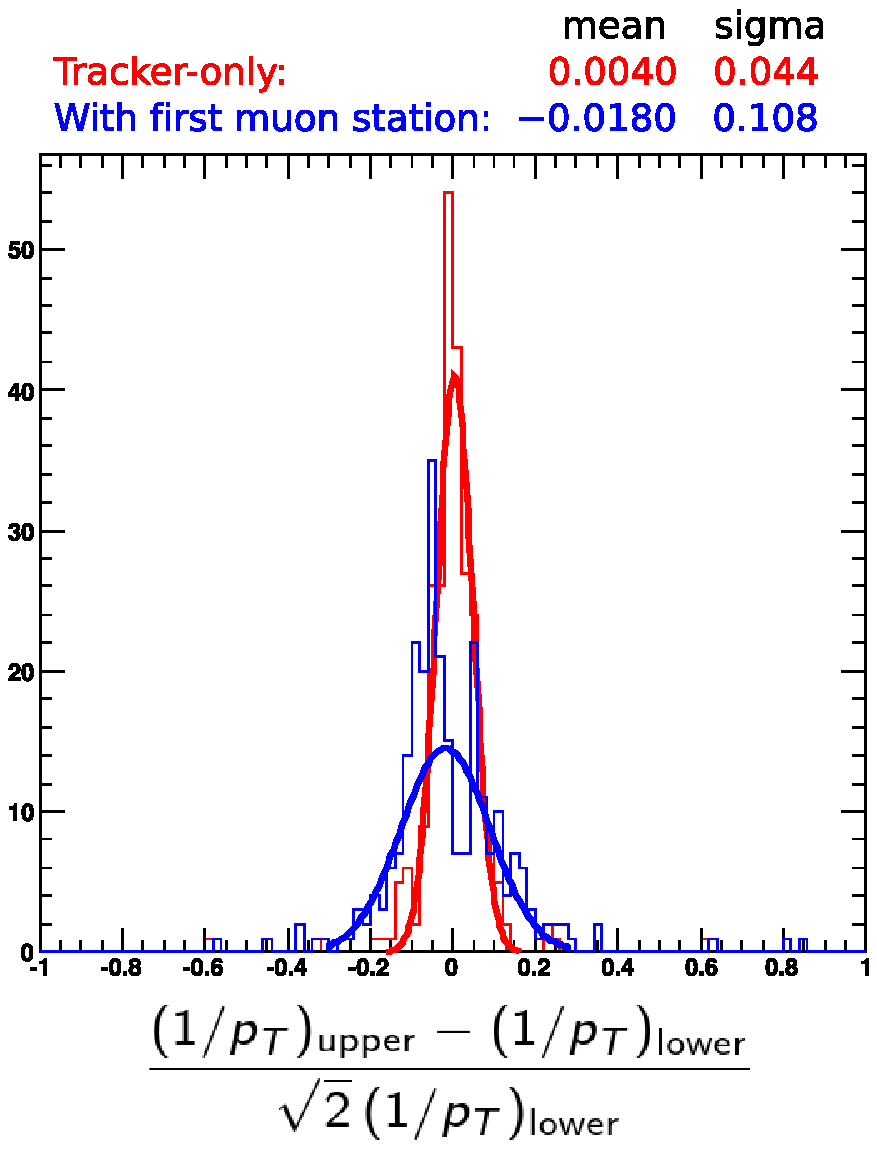
\includegraphics[width=\linewidth]{without_alignment.pdf}
\end{center}
\column{0.4\linewidth}
\begin{center}
\textcolor{darkblue}{After muon alignment}

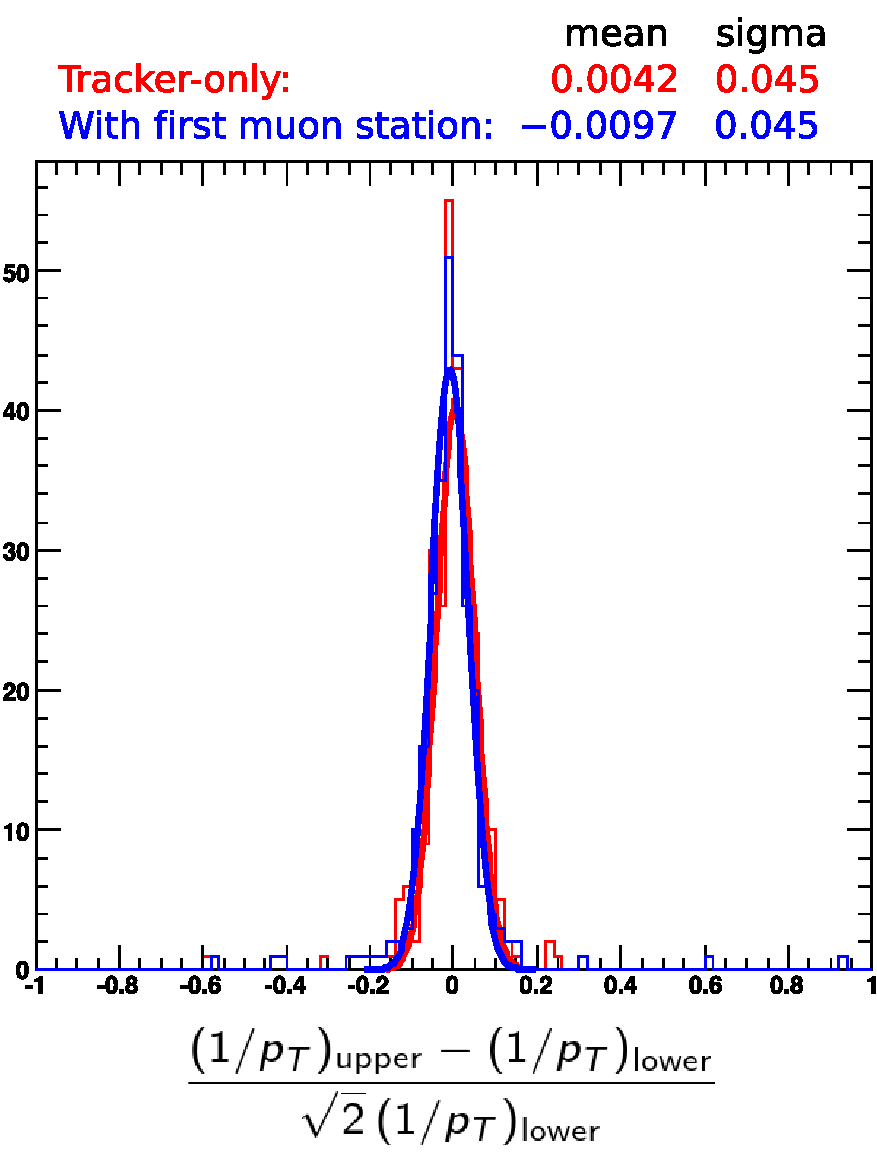
\includegraphics[width=\linewidth]{with_alignment.pdf}
\end{center}

\column{0.3\linewidth}
\mbox{ }

\vspace{0.15 cm}
\scriptsize \centering \textcolor{darkblue}{Plot from Technical Design Report}

\textcolor{darkblue}{(no misalignment)}

\vspace{0.2 cm}
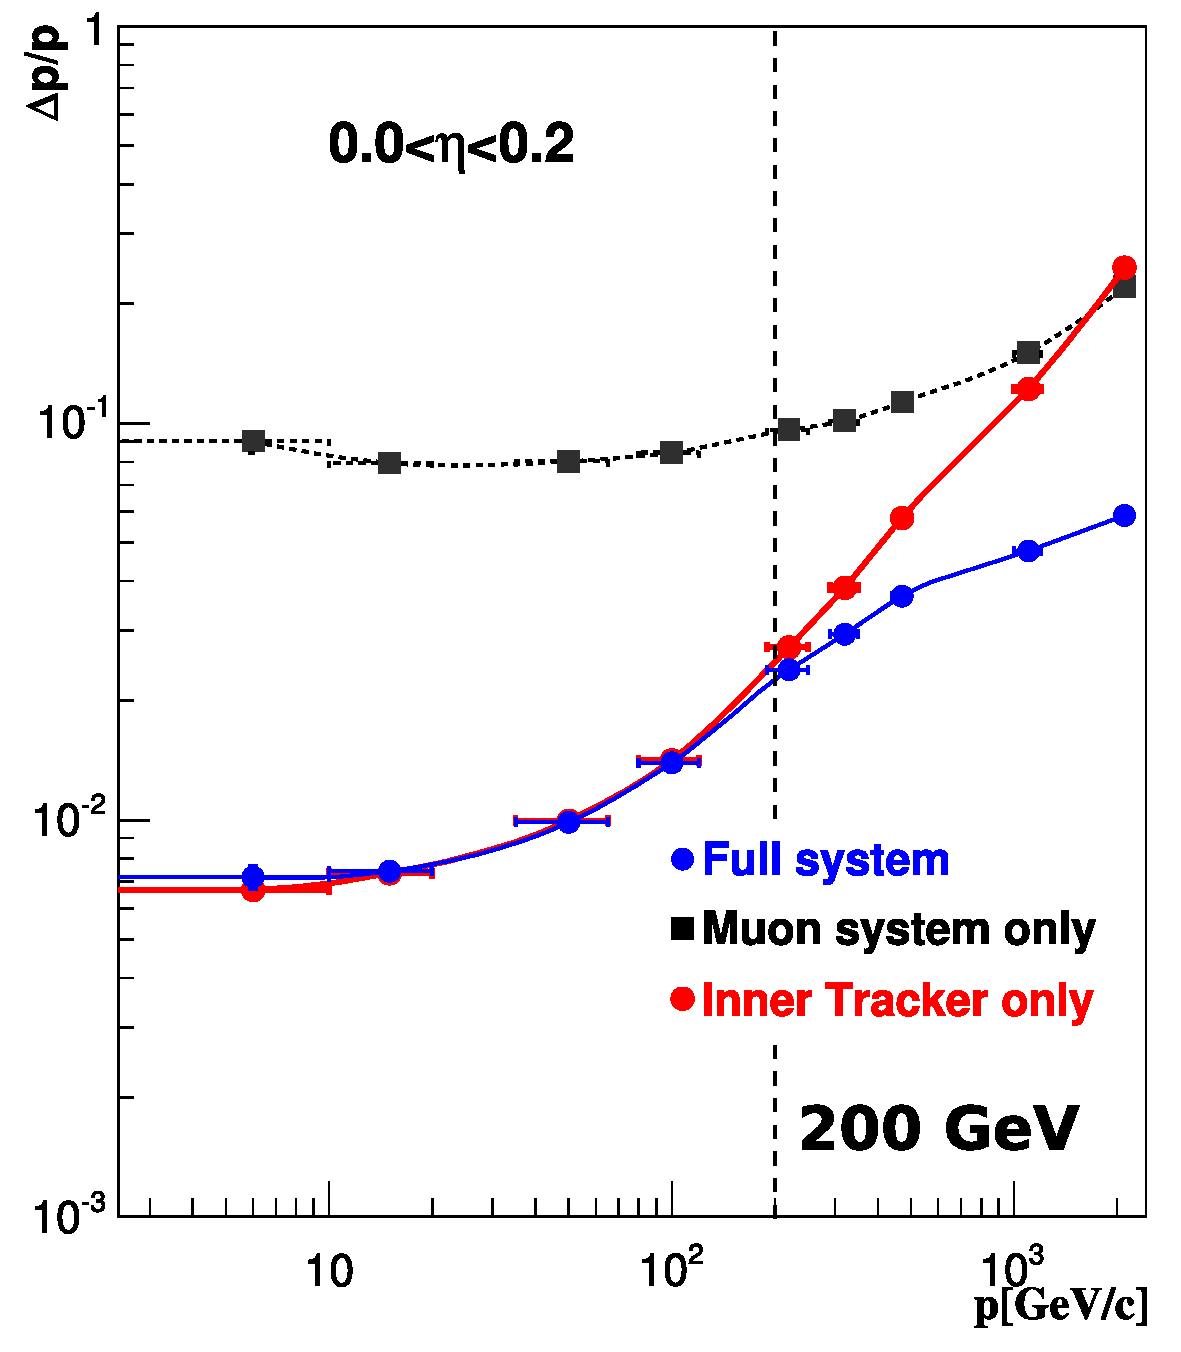
\includegraphics[width=\linewidth]{Figure_001-005-a.pdf}

sigma $\sim$ 0.025 at 200~GeV for a perfect detector
\end{columns}
\end{frame}

%% \section*{First section}
%% \begin{frame}
%% \begin{center}
%% \Huge \textcolor{blue}{First section}
%% \end{center}
%% \end{frame}

\begin{frame}
\frametitle{Conclusions}

\begin{itemize}\setlength{\itemsep}{0.5 cm}
\item Alignment strategy tailored to unique characteristics of the CMS muon system
\item Procedures are well-understood in Monte Carlo, with reasonably good agreement with data
\item Different methods based on global and local data for cross-checks
\item Demonstrated excellent performance in beam-halo and cosmic rays: a good sign for alignment with first collisions!
\end{itemize}

\label{numpages}
\end{frame}

\end{document}
